%
% Example document for using the hhuBeamer-class.
% PLEASE read carefully.
%

% You can change fontsize here - the titlepage has fixed font size
\documentclass[11pt]{beamer}

% you can switch between "english" and "german"
% there might be some babel-error on the first compile time
% but normally it can be ignored
% Use frametitlestandard for standard psoition of frametitle
% or framtetitletop for top-position of frametitle
\usetheme[english,frametitletop]{hhu}

%
% Note: Use \hhu to insert the correct spelling of the HHU's name
% Note: Use \noframetitle for frames without title
% Note: Use \begin{highlighted}...\end{highlighted} to emphasize formulas
% Note: There are predefined colors hhuX with 
%		X = Blue,Green,Red,Orange,Darkblue,Iceblue,Turquoise,Black.
%		Please use only these colors and use hhuBlack and hhuBlue
%		as standard colors.
%
%

\usepackage{minted}

% https://gist.github.com/mutbuerger/e65575180b99e9074129
\usepackage{tcolorbox}
\usepackage{multimedia}
\tcbuselibrary{skins, breakable}
\usetikzlibrary{shadings, backgrounds}
\newtcolorbox{codeblock}[2][]
{%
	enhanced,
	colbacktitle=titlebg,
	coltitle=titlecolor,
	interior style={%
		top color=codebg,
		bottom color=codebg
	},
	boxrule=0mm,
	arc=0.6mm,
	width= (\linewidth),
	fonttitle=\footnotesize,
	adjusted title=\texttt{#1},
	after title={%
		\hfill\setlength{\fboxsep}{2pt}
		\colorbox{languagebg}{\textcolor{black}
			{\footnotesize{\texttt{#2}}}}
	},
	overlay={%
		\begin{tcbclipinterior}\fill[numberbg] (frame.south west)
			rectangle ([xshift=5mm]frame.north west);
		\end{tcbclipinterior}
	},
	top=0mm,
	bottom=0mm,
	left=5mm,
	right=0mm
}

\newtcolorbox{terminalblock}[1][]
{%
	enhanced,
	colbacktitle=titlebg,
	coltitle=titlecolor,
	interior style={%
		top color=termbg,
		bottom color=termbg
	},
	boxrule=0mm,
	arc=0.6mm,
	width= (\linewidth),
	fonttitle=\footnotesize,
	top=1mm,
	bottom=0mm,
	left=1mm,
	right=1mm
}

\newmintedfile{cpp}{
	linenos,
	autogobble,
	breaklines=true,
	breaksymbol=,
	breakindent=4mm,
	breakbefore=.,
	breakbeforesymbolpre=,
	breakbeforesymbolpost=,
	baselinestretch=0.8,
	framesep=5mm,
	numbersep=7pt,
	fontsize=\footnotesize,
	style=manni
}

\newmintedfile{text}{
	autogobble,
	breaklines=true,
	breaksymbol=,
	breakindent=4mm,
	breakbefore=.,
	breakbeforesymbolpre=,
	breakbeforesymbolpost=,
	baselinestretch=0.8,
	framesep=5mm,
	fontsize=\footnotesize
}

\AtBeginEnvironment{terminalblock}{\color{white}}

\title{hhuOS}
\date{13.07.2023\\Institute of Computer Science \\Heinrich Heine University Düsseldorf}
\author{Christian Gesse, Fabian Ruhland}
\institute{}

\begin{document}
	
	\frame[plain]{\maketitle}
	
	\section{Introduction}
	
	\begin{frame}{Facts about hhuOS}
	\begin{itemize}
		\setlength\itemsep{1em}
		\item A small operating system for teaching and learning purposes
		\item written for x86 32-bit architecture
		\item written in C++ and x86-Assembler using gcc and nasm
		\item Open-Source, published under the GPL v3 license
		\item $\sim25000$ lines of code
	\end{itemize}
	\end{frame}
	
	\begin{frame}{hhuOS - Features}
		\begin{itemize}
			\item Processes \& Threads
			\begin{itemize}
				\item Round-Robin based preemptive scheduling
				\item Binary files are executed as processes
				\item Each process has its own address space
			\end{itemize}
			\pause
			\item Adress spaces and memory management
			\begin{itemize}
				\item Using x86-Paging mechanism (virtual/physical memory)
				\item Lazy mapping implementation
				\item Kernel address space is always mapped at 3 GiB (not accessible from user space)
				\item Different memory managing algorithms are implemented (Free List, Bitmap, Table)
			\end{itemize}
		\end{itemize}
	\end{frame}

	\begin{frame}{hhuOS - Features}
		\begin{itemize}
			\item Unified Library
			\begin{itemize}
				\item Single codebase for user- and kernel-space library
				\item Functions requiring kernel access are outsourced into an interface (implemented two times - for kernel and user space)
				\item Kernel access from user space via system calls (software interrupts)
			\end{itemize}
			\pause
			\item Further features
			\begin{itemize}
				\item Virtual Filesystem (can mount physical filesystems)
				\item Hardware support (Keyboard, PCI, Floppy AHCI, VESA \& CGA Graphics)
				\item Multiboot compatible: Bootable on UEFI and BIOS systems (BIOS calls are supported)
				\item Own UEFI bootloader (towboot, developed by Niklas Sombert)
				\item Experimental support for networking, thanks to several bachelors thesis (2 drivers and a UDP/IP Stack)
			\end{itemize}	
		\end{itemize}
	\end{frame}
	
	\section{Memory \& Paging}

\begin{frame}{Overview: Memory \& Paging}
	\begin{itemize}
		\setlength\itemsep{1em}
		\item Paging: Abstract physical memory from virtual address spaces
		\item New pages can be mapped in/out dynamically
		\item Use of different address spaces for process separation
		\item Kernel is mapped at 3 GiB $\rightarrow$ Higher-Half-Kernel (always visible)
		\item Adresses below 3 GiB are used for user space memory
	\end{itemize}	
\end{frame}

\begin{frame}{Paging: The boot process}
	\begin{itemize}
		\item How to allocate memory when no memory manager is available?
		\item How to map the Kernel-code at 3 GiB without losing the EIP?
		\item Solution: Activate paging in several steps
	\end{itemize}
	\pause
	\begin{figure}
		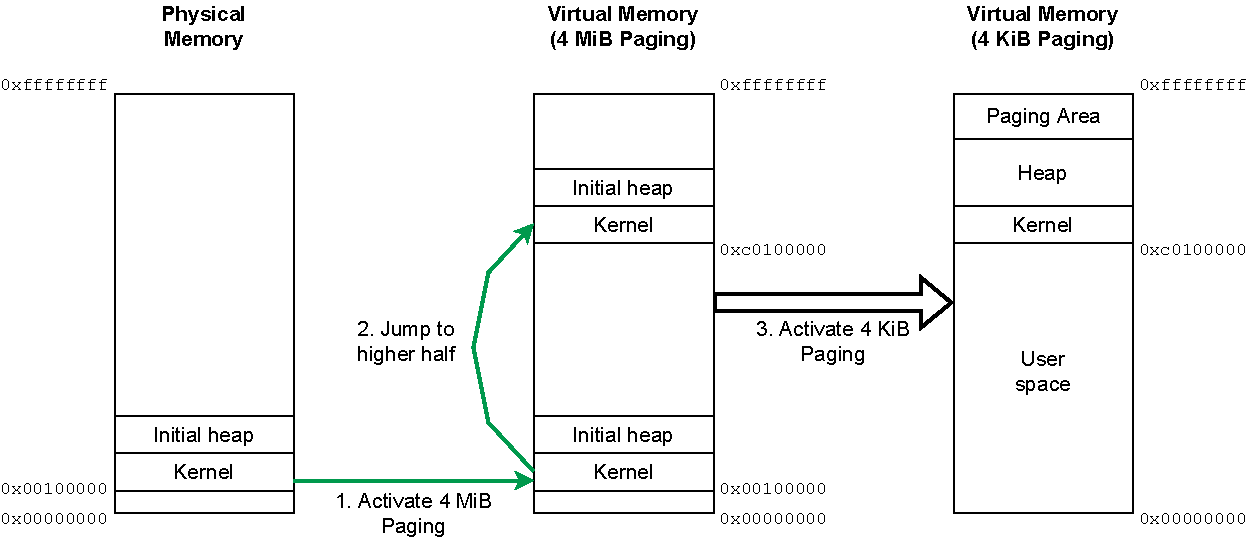
\includegraphics[width=0.9\textwidth]{img/paging}
	\end{figure}
\end{frame}

\begin{frame}{Allocating heap memory}
	\begin{enumerate}
		\setlength\itemsep{1em}
		\item Invoke Free list manager to find free memory block in heap
		\item Slice free block (with respect to alignment)
		\item Return pointer to found block
		\item If the block was not previously mapped, the first access will generate a pagefault
		\item Fault handler is invoked during interrupt handling
		\item Search unused pageframe and map it to the virtual fault address
		\item Return to program
	\end{enumerate}
\end{frame}
	
	\section{Processes \& Threads}

\begin{frame}{Process Scheduling}
	\begin{itemize}
		\setlength\itemsep{1em}
		\item Global scheduler manages threads in a queue
		\item Timer invokes scheduler every 10ms to switch to next thread
		\begin{itemize}
			\item If current and next threads belong to different processes, address space needs to be switched
		\end{itemize}
		\item Threads can be blocked and unblocked by other threads
		\item Threads can sleep for a defined time
		\begin{itemize}
			\item Scheduler manages sleeping threads in a separate queue
		\end{itemize}
		\item It is possible to join other threads (or processes)
		\begin{itemize}
			\item Each thread has a list of joining threads, that are reassigned to the scheduler, once the thread has finished
		\end{itemize}
	\end{itemize}	
\end{frame}


	\section{Filesystem}

\begin{frame}{Storage Devices}
	\begin{itemize}
		\setlength\itemsep{1em}
		\item \textit{StorageDevice} as interface for block devices
		\item Only 4 methods: \textit{getSectorCount()}, \textit{getSectorSize()}, \textit{read()}, \textit{write()}
		\item Implemented for IDE (hard drives), Floppy, Virtual Drives, and Partitions
	\end{itemize}	
\end{frame}

\begin{frame}{Virtual File System}
	\begin{itemize}
		\setlength\itemsep{1em}
		\item Overlay over physical file systems (e.g. FAT)
		\item Storage devices can be mounted to any folder
		\item Files and directories are represented by \texttt{Filesystem::Node} (similar to \textit{INode})
		\item Interface \texttt{Filesystem::Driver} for physical file systems
		\item Implemented using \textit{FatFs}\footnotemark[1] to support all FAT variants
	\end{itemize}
	\vspace{3.0em}
	\footnotemark[1]\footnotesize{\url{http://elm-chan.org/fsw/ff/00index_e.html}}
\end{frame}

	
	\section{Game library}

\begin{frame}{2D games}
	\begin{itemize}
		\item 2D game library implemented by Malte Sehmer (bachelor thesis)
		\item Supports sprites (loaded from bitmap files) and animations
		\item Collision detection based on rectangle colliders (polygon colliders are conceptually implemented)
		\item Linear and accelerated movements are implemented (e.g. gravity)
		\item Particle system (bachelor thesis by Abdulbasir Gümüs)
	\end{itemize}
	\begin{minipage}{0.49\textwidth}
		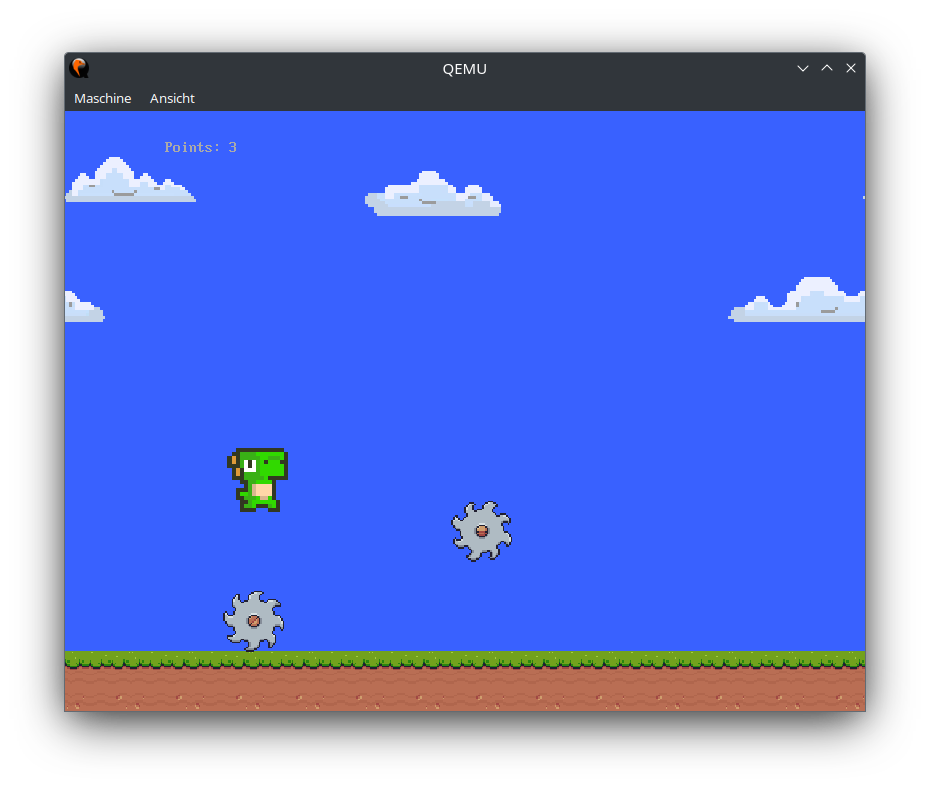
\includegraphics[width=0.9\textwidth]{img/dino}
	\end{minipage}
	\begin{minipage}{0.49\textwidth}
	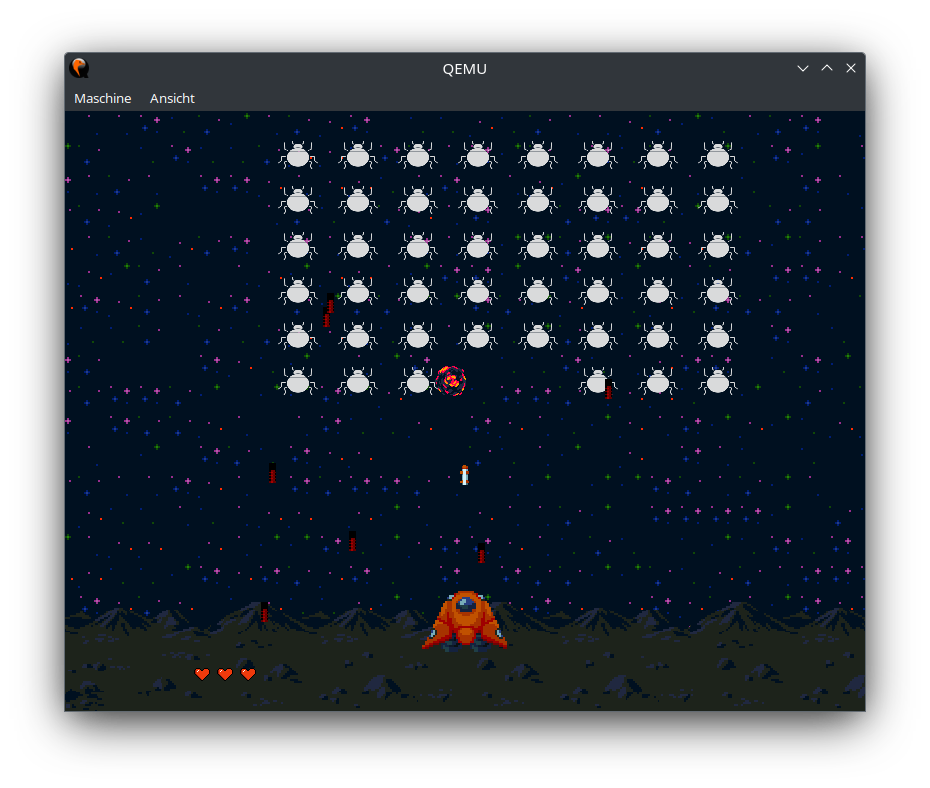
\includegraphics[width=0.9\textwidth]{img/bug}
	\end{minipage}
	\pause
	\begin{center}
		\textbf{But can it run Crysis?}
	\end{center}
\end{frame}

\begin{frame}{3D games - Work in Progress}
	\begin{itemize}
		\item 3D extension to the game library (bachelor thesis by Richard Schweitzer)
		\item Supports wireframe 3D-objects loaded from OBJ files
		\item Collision detection based on spheres
		\item Many features are missing (e.g. texturing, z-buffering, etc.)
	\end{itemize}
	\begin{minipage}{0.49\textwidth}
		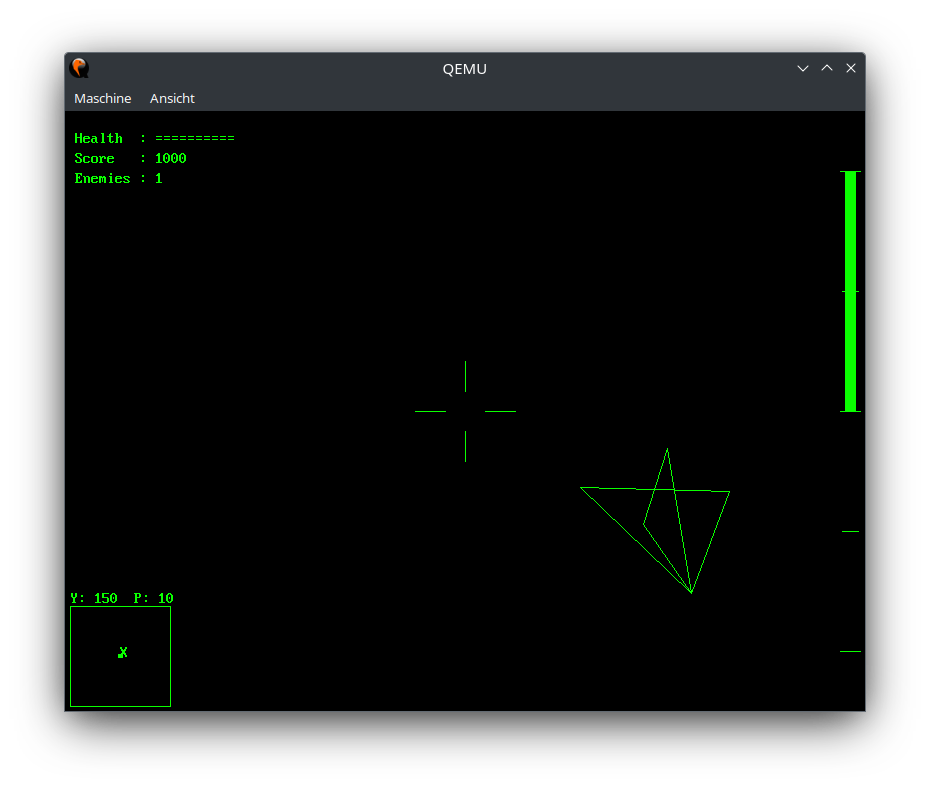
\includegraphics[width=0.95\textwidth]{img/battlezone1}
	\end{minipage}
	\begin{minipage}{0.49\textwidth}
		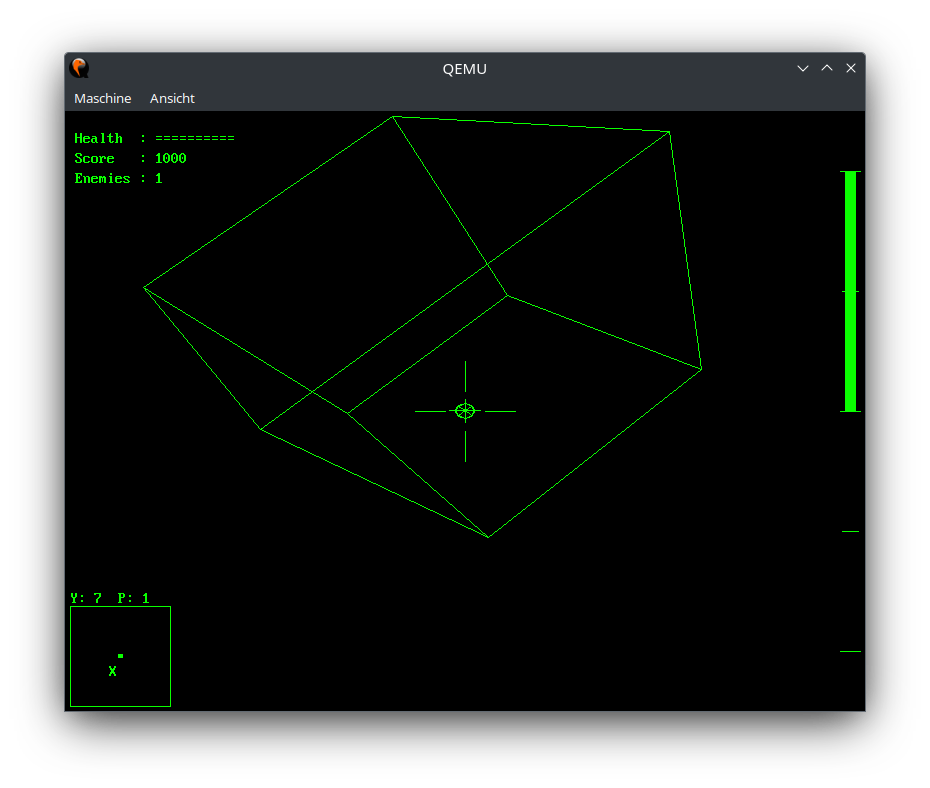
\includegraphics[width=0.95\textwidth]{img/battlezone2}
	\end{minipage}
\end{frame}

	
	\section{Future Work}

\begin{frame}{Future Work}
	\begin{itemize}
		\setlength\itemsep{1em}
		\item Implement more device drivers (sound, graphics, network, etc.)
		\item Enhance network stack
		\item Better scheduling (priorities, I/O management)
		\item New (custom) filesystems
		\item Multicore support
		\item Support modern x86-Features (Physical Address Extensions, Long mode, SSE, etc.)
	\end{itemize}	
\end{frame}
	
	%\begin{frame}[standout]{Demo}
	%	\begin{center}
	%		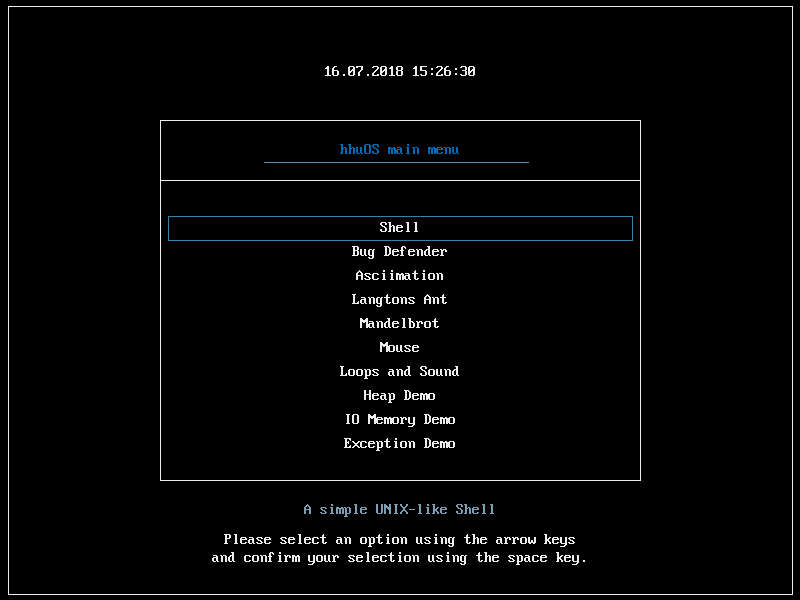
\includegraphics[width=.6\textwidth]{img/hhuos_main}
	%	\end{center}	
	%\end{frame}

\end{document}